\begin{figure*}[t!]
    \centering
    ~ 
    \begin{subfigure}[t]{0.3\textwidth}
        \centering
        
\includegraphics[height=1.2in]{julia_01.png}
        \caption{$c=0.1$.}
    \end{subfigure}	
	~
    \begin{subfigure}[t]{0.2\textwidth}
        \centering
        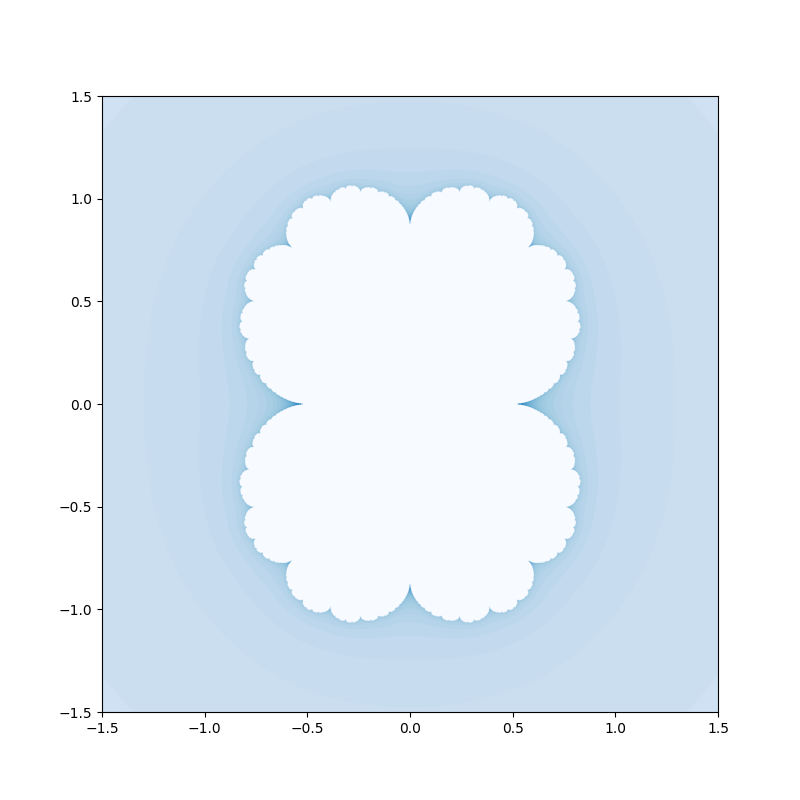
\includegraphics[height=1.2in]{cauliflower.png}
        \caption{$c=1/4$, the Cauliflower.}
    \end{subfigure}%
    ~ 
    \begin{subfigure}[t]{0.3\textwidth}
        \centering
        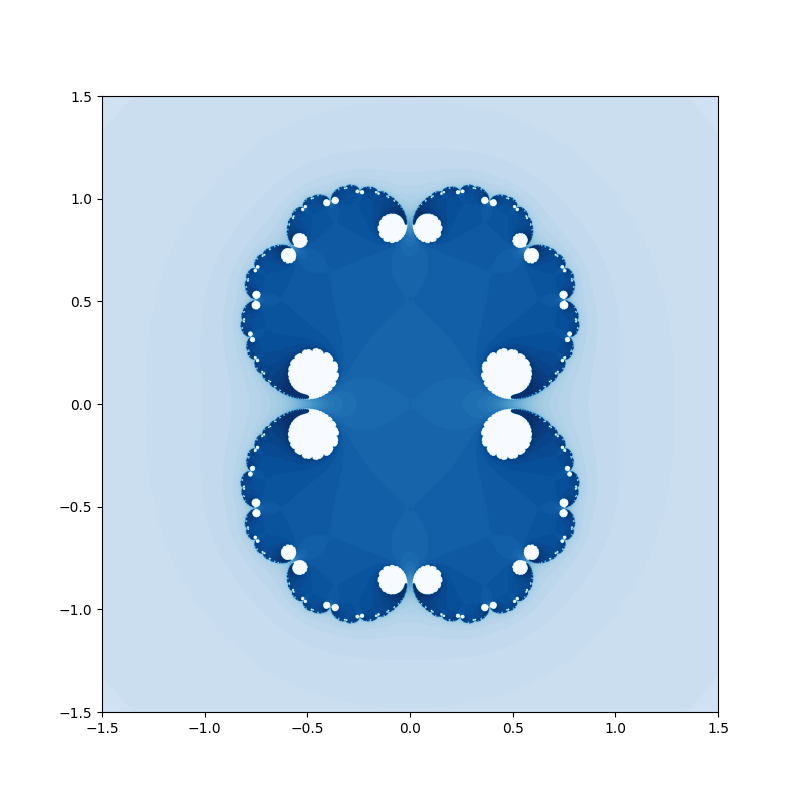
\includegraphics[height=1.2in]{julia_026.png}
        \caption{$c=0.26$.}
    \end{subfigure}
    \caption{The Julia set $\mathcal J_c$ of $f_c$ for different values of $c$. When $c>1/4$, the Julia set is no longer connected.}
\end{figure*}
